% Pengaturan ukuran teks dan jenis dokumen
\documentclass[11pt]{article}

% Pengaturan ukuran halaman dan margin
\usepackage[a4paper,top=30mm,left=30mm,right=20mm,bottom=20mm]{geometry}

% Pengaturan ukuran spasi
\usepackage[singlespacing]{setspace}

% Judul dokumen
\title{Proposal Tugas Akhir ITS}
\author{Musk, Elon Reeve}

% Pengaturan format bahasa
\usepackage[indonesian]{babel}

% Pengaturan detail pada file PDF
\usepackage[pdfauthor={\@author},bookmarksnumbered,pdfborder={0 0 0}]{hyperref}

% Pengaturan jenis karakter
\usepackage[utf8]{inputenc}

% Pengaturan ukuran indentasi
\setlength{\parindent}{2em}

% Package lainnya
\usepackage{etoolbox} % Mengubah fungsi default
\usepackage{enumitem} % Pembuatan list
\usepackage{lipsum} % Pembuatan template kalimat
\usepackage{graphicx} % Input gambar
\usepackage{longtable} % Pembuatan tabel
\usepackage[table,xcdraw]{xcolor} % Pewarnaan tabel
\usepackage[numbers]{natbib} % Kutipan artikel
\usepackage{changepage} % Pembuatan teks kolom
\usepackage{multicol} % Pembuatan kolom ganda
\usepackage{multirow} % Pembuatan baris ganda
\usepackage{float}
\usepackage{outlines}

% Pengaturan format judul bab
\usepackage{titlesec}
\renewcommand{\thesection}{\arabic{section}}
\titleformat*{\section}{\normalsize\bfseries}
\titleformat*{\subsection}{\normalsize\bfseries}
\titlespacing{\section}{0ex}{3ex}{1.5ex}
\titlespacing{\subsection}{0ex}{3ex}{1.5ex}

% Isi keseluruhan dokumen
\begin{document}

  % Menonaktifkan penomoran halaman
  \pagenumbering{gobble}

  % Lembar pengesahan
  \begin{flushleft}
    % Ubah kalimat berikut sesuai dengan nama departemen dan fakultas
    \textbf{Departemen Teknik Komputer - FTEIC}\\
    \textbf{Institut Teknologi Sepuluh Nopember}\\
  \end{flushleft}
  
  \begin{center}
    % Ubah detail mata kuliah berikut sesuai dengan yang ditentukan oleh departemen
    \underline{\textbf{EC184701 - PRA TUGAS AKHIR (2 SKS)}}
  \end{center}
  
  \begin{adjustwidth}{-0.2cm}{}
    \begin{tabular}{lcp{0.7\linewidth}}
  
      % Ubah kalimat-kalimat berikut sesuai dengan nama dan NRP mahasiswa
      Nama Mahasiswa &:& Fathullah Auzan Setyo Laksono \\
      Nomor Pokok &:& 07211840000053 \\
  
      % Ubah kalimat berikut sesuai dengan semester pengajuan proposal
      Semester &:& Ganjil 2021/2022 \\
  
      % Ubah kalimat-kalimat berikut sesuai dengan nama-nama dosen pembimbing
      Dosen Pembimbing &:& 1. Reza Fuad Rachmadi, S.T., M.T., Ph.D. \\
      & & 2. Dr. Eko Mulyanto Yuniarno, S.T., M.T. \\
  
      % Ubah kalimat berikut sesuai dengan judul tugas akhir
      Judul Tugas Akhir &:& \textbf{Estimasi Umur, Gender dan Etnik Menggunakan} \\
      & & \textbf{Covolutional Neural Network Berbasis Citra Wajah} \\
  
      Uraian Tugas Akhir &:& \\
    \end{tabular}
  \end{adjustwidth}
  
  % Ubah paragraf berikut sesuai dengan uraian dari tugas akhir
  Fitur wajah seperti identifikasi umur, gender dan etnik dapat sangat berguna dalam banyak pengimplementasian ilmu seperti pengamatan visual, diagnosa medis, sistem interaksi komputer manusia, biometric, pengumpulan informasi, penegakan hukum, pemasaran dan banyak lainnya. Dimana sebagian besar data mengenai fitur wajah tersebut masih diambil secara manual melalui survei ataupun pengamatan pada banyak individu. Berdasarkan World Population Clock pada websitenya, di dunia terdapat lebih dari 7 miliar orang yang tersebar di berbagai macam pulau dan benua. Jumlah tersebut masih terus bertambah sampai sekarang. Dimana di setiap benua dan negara tersebut terdapat berbagai karakteristik dan ciri manusia yang berbeda dengan kata lain Etnik yang berbeda-beda. Dengan banyaknya jumlah penduduk dan keberagamannya tersebut, jika data fitur wajah diambil secara manual akan memakan waktu dan tenaga yang banyak. Oleh karena itu perlu dibuat suatu sistem yang dapat mengestimasi umur, gender dan etnik serta mengyimpan penghitungan datanya untuk mempermudah pengumpulan data. Dimana kamera akan menangkap gambar dari seseorang dan dilakukan proses estimasi umur, gender dan etnik yang kemudian datanya disimpan untuk digunakan kedepannya.
  \vspace{1ex}
  
  \begin{flushright}
    % Ubah kalimat berikut sesuai dengan tempat, bulan, dan tahun penulisan
    Surabaya, Desember 2021
  \end{flushright}
  \vspace{1ex}
  
  \begin{center}
  
    \begin{multicols}{2}
  
      Dosen Pembimbing 1
      \vspace{12ex}
  
      % Ubah kalimat-kalimat berikut sesuai dengan nama dan NIP dosen pembimbing pertama
      \underline{Dr. I Ketut Eddy Purnama, S.T., M.T.} \\
      NIP. 196907301995121001
  
      \columnbreak
  
      Dosen Pembimbing 2
      \vspace{12ex}
  
      % Ubah kalimat-kalimat berikut sesuai dengan nama dan NIP dosen pembimbing kedua
      \underline{Reza Fuad Rachmadi S.T., M.T., Ph.D.} \\
      NIP. 198504032012121001
  
    \end{multicols}
    \vspace{6ex}
  
    Mengetahui, \\
    % Ubah kalimat berikut sesuai dengan jabatan kepala departemen
    Kepala Departemen Teknik Komputer FTEIC - ITS
    \vspace{12ex}
  
    % Ubah kalimat-kalimat berikut sesuai dengan nama dan NIP kepala departemen
    \underline{Dr. Supeno Mardi Susiki Nugroho, S.T., M.T.} \\
    NIP. 197003131995121001
  
  \end{center}
  \newpage

  \begin{center}
    % Ubah judul
    \textbf{Convolutional Neural Network untuk Estimasi Umur, Gender dan Etnik Berbasis Citra Wajah}
  \end{center}

  % Konten pendahuluan
  \section{PENDAHULUAN}

\subsection{Latar Belakang}

% Ubah paragraf-paragraf berikut sesuai dengan latar belakang dari tugas akhir
Penyakit yang menyerang otak merupakan salah satu penyakit yang dapat menyebabkan manusia kehilangan kemampuan kritikalnya dalam menjalani kehidupan sehari-hari, seperti berbicara, berpikir, atau bahkan dapat menyebabkan kematian. Pada tahun 2007 berdasarkan World Health Organization (WHO) terdapat sekitar 1 miliar orang yang menderita penyakit otak, mulai dari Migrain hingga penyakit seperti Parkinson.[1] Terdapat berbagai macam jenis penyakit yang menyerang otak seperti, Alzheimer, Tumor, dan Stroke. Penyakit-penyakit ini dapat berakibat fatal apabila tidak ditangani dengan cepat, sehingga pendeteksian awal  terhadap penyakit-penyakit ini diperlukan untuk mencegah penyakit tersebut semakin memburuk.

Magnetic Resonance Imaging (MRI) merupakan salah satu metode yang digunakan secara luas dalam mendeteksi kondisi abnormal pada organ manusia seperti otak (Legaz-Aparicio et al., 2017, Olson and Perry, 2013).[2][3] Metode ini semakin banyak digunakan karena karakteristiknya yang tidak berbahaya pada manusia dan dapat menghasilkan gambar dengan tingkat kontras yang tinggi (Akkus et al., 2017).[4] Perangkat Magnetic Resonance (MR) menggunakan magnet yang kuat dan sinyal frekuensi radio sebagai ganti metode radiasi ionisasi untuk menghasilkan gambar kondisi otak.

Diagnosis penyakit otak dengan menggunakan MRI masih dapat dilakukan secara manual oleh radiologist dengan membaca hasil citra MRI. Berdasarkan jurnal American College of Radiology, hasil citra MRI dapat diinterpretasikan oleh radiologist dalam waktu 24 jam.[5] Pembacaan citra MRI masih bergantung terhadap kemampuan dan data yang dimiliki oleh seorang radiologist. Apabila hasil citra MRI dikeluarkan dengan cepat tanpa melalui analisa yang cukup, maka pembacaan citra MRI tersebut dapat menyebabkan kesalahan diagnosis. Namun, apabila hasil citra MRI dikeluarkan terlalu lama, maka dapat berakibat buruk pada kondisi pasien yang membutuhkan perawatan secepat mungkin.

Deep learning merupakan salah satu metode yang banyak digunakan dalam penelitian mengenai klasifikasi dan segmentasi dari citra MRI otak (Akkus et al., 2017; Bernal et al. 2018).[4][6] Metode deep learning banyak digunakan karena dapat menghasilkan hasil yang akurat untuk masalah kompleks yang membutuhkan banyak data. Salah satu metode deep learning yang digunakan dalam klasifikasi citra MRI adalah dengan menggunakan Convolutional Neural Network (CNN).


\subsection{Rumusan Masalah}

% Ubah paragraf berikut sesuai dengan rumusan masalah dari tugas akhir
Hasil pembacaan citra MRI secara konvensional oleh dokter radiologi bergantung pada jumlah data yang dimiliki dan kemampuan analisa dokter radiologi. Metode pembacaan secara konvesional ini sangat rentan terhadap human error. Kesalahan diagnosis kondisi otak dapat berakibat buruk terhadap pasien, dimana perawatan yang didapatkan oleh pasien tidak sesuai dengan kondisi pasien tersebut.

\subsection{Penelitian Terkait}

% Ubah paragraf berikut sesuai dengan penelitian lain yang terkait dengan tugas akhir
Pada tahun 2019, Muhammad Talo dan rekan-rekannya mempublikasikan sebuah paper mengenai penelitian mereka mengenai klasifikasi penyakit otak dengan menggunakan 2D CNN. Pada penelitian tersebut mereka menggunakan metode transfer learning dari pre-trained model seperti: ResNet, Vgg-16, dan AlexNet. Pada penelitian tersebut mereka berhasil mengklasifikasikan 5 jenis kondisi otak (Normal, Cerebovascular, Neoplastic, Degenerative, dan Infectious) dan ResNet-50 mendapatkan hasil terbaik dengan tingkat akurasi mencapai 95%.[7]
 
Pada bulan Agustus 2021, Juezhao Yu., Et al. mempublikasikan sebuah paper dengan judul “2D CNN vs 3D CNN for False-Positive Reduction in Lung Cancer Screening”. Pada research tersebut mereka melakukan percobaan dengan menggunakan citra MRI untuk kanker paru-paru dan meneliti apakah 3D CNN dapat mengurangi nilai false-positive apabila dibandingkan dengan 2D CNN. Pada penelitian tersebut mereka berhasil mendapatkan bahwa  3D CNN berhasil mengurangi nilai false-positive sebanyak 2%.[8]

\subsection{Gap Penelitian}
Penelitian mengenai klasifikasi penyakit otak  menggunakan CNN masih menggunakan metode 2D CNN, namun belum terdapat penelitian mengenai klasifikasi penyakit otak menggunakan 3D CNN.

\subsection{Tujuan Penelitian}

% Ubah paragraf berikut sesuai dengan tujuan penelitian dari tugas akhir
Penelitian ini bertujuan untuk dapat mengembangkan sebuah sistem yang dapat mengklasifikasikan 4 tipe kondisi otak, yaitu 1 kondisi otak normal dan 3 lainnya merupakan kondisi berpenyakit seperti: Alzheimer, Tumor dan Stroke dengan menggunakan metode 3D CNN pada deep learning.

  % Konten tinjauan pustaka
  \section{TINJAUAN PUSTAKA}

% Ubah konten-konten berikut sesuai dengan isi dari tinjauan pustaka
Tujuan yang ingin dicapai dari Tugas Akhir ini adalah untuk mengembangkan sebuah model menggunakan 
Convolutional Neural Network yang dapat mengestimasi umur, gender dan etnik yang mempermudah proses 
pengumpulan dan pengambilan data terkait umur, gender dan etnik.

\subsection{Wajah}

% Contoh penggunaan referensi dari pustaka
% Newton pernah merumuskan \citep{Newton1687} bahwa \lipsum[8]
% Contoh penggunaan referensi dari persamaan
% Kemudian menjadi persamaan seperti pada persamaan \ref{eq:FirstLaw}.

Wajah merupakan bagian dari tubuh manusia yang menjadi fokus perhatian di dalam interaksi sosial, 
wajah memainkan peranan vital dengan menunjukan identitas dan emosi. Kemampuan manusia untuk mengetahui 
seseorang dari wajahnya sangat luar biasa. Kita dapat mengenali ribuan wajah karena frekuensi interaksi 
yang sangat sering ataupun hanya sekilas bahkan dalam rentang waktu yang sangat lama. Bahkan kita mampu 
mengenali seseorang walaupun terjadi perubahan pada orang tersebut karena bertambahnya usia atau 
pemakaian kacamata atau perubahan gaya rambut. Oleh karena itu wajah digunakan sebagai organ dari tubuh 
manusia yang dijadikan indikasi pengenalan seseorang. Dimana identitas, ekspresi, gender, umur dan etnik 
disebut dengan dalam wajah.

\subsection{Umur}
Umur merupakan rentang kehidupan yang diukur dengan tahun, dikatakan masa awal dewasa adalah usia 18 – 40 
tahun, dewasa madya adalah 41 – 60 tahun, dewasa lanjut lebih dari 60 tahun. Umur adalah lamanya hidup 
dalam tahun yang dihitung sejak dilahirkan.
% input gambar
\begin{figure} [H] \centering
    % Nama dari file gambar yang diinputkan
    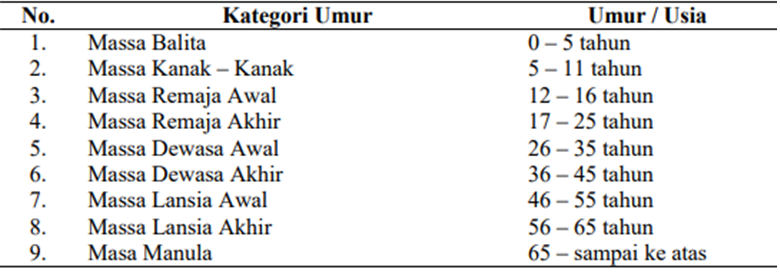
\includegraphics[scale=0.6]{gambar/umur.png}
    % Keterangan gambar yang diinputkan
    \caption{Kategori umur menurut Depkes. RI (2009)}
    % Label referensi dari gambar yang diinputkan
    \label{fig:Umur}
\end{figure}

\subsection{Gender}
Gender merupakan perbedaan yang terlihat antara laki-laki dan perempuan apabila dilihat dari penampilan 
dan tingkah laku. Gender dapat didefinisikan sebagai keadaan dimana individu yang lahir secara biologis 
sebagai laki-laki dan perempuan yang kemudian memperoleh pencirian sosial sebagai laki-laki dan perempuan 
melalui atribut maskulinitas dan feminimitas yang diperlihatkan individu tersebut.

\subsection{Etnis}
Kata etnis mengacu pada suatu golongan atau kelompok manusia yang anggota - anggotanya mengidentifikasikan 
dirinya dengan sesamanya, biasanya berdasarkan garis keturunan dan adat yang dianggap sama. Identitas 
etnis ditandai oleh pengakuan dari orang lain akan ciri khas kelompok tersebut seperti kesamaan budaya, 
bahasa, agama, perilaku, dan ciri-ciri biologis.
% input gambar
\begin{figure} [H] \centering
    % Nama dari file gambar yang diinputkan
    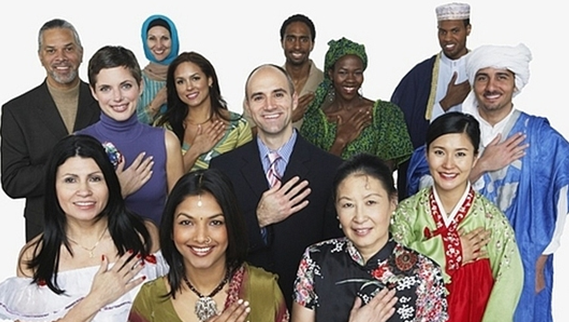
\includegraphics[scale=0.6]{gambar/etnik.png}
    % Keterangan gambar yang diinputkan
    \caption{Macam-macam Etnik di dunia}
    % Label referensi dari gambar yang diinputkan
    \label{fig:Etnik}
\end{figure}

\subsection{Visi Komputer}
Visi komputer adalah bidang ilmiah interdisipliner yang membahas bagaimana komputer dapat memperoleh 
pemahaman tingkat tinggi dari gambar atau video digital. Dari perspektif teknik, bidang ini berupaya 
mengotomatiskan tugas-tugas yang dapat dilakukan oleh sistem pengelihatan  manusia. Tugas  penglihatan 
komputer   meliputi metode untuk memperoleh, memproses, menganalisis dan memahami gambar digital, dan 
ekstraksi data dimensi tinggi dari dunia nyata untuk menghasilkan informasi numerik atau simbolis, 
misalnya dalam bentuk keputusan. Pengertian dalam konteks ini berarti transformasi gambar visual 
(input retina) menjadi deskripsi mengenai dunia sekitar yang dapat berinteraksi dengan proses pemikiran 
lain dan memperoleh tindakan yang sesuai. Pemahaman gambar ini dapat dilihat sebagai penguraian informasi 
simbolik dari data gambar menggunakan model yang dibangun dengan bantuan geometri, fisika, statistik, dan 
teori pembelajaran. Sub-domain dari pengelihatan komputer meliputi rekonstruksi adegan, deteksi peristiwa, 
pelacakan video, pengenalan objek, estimasi pose 3D, pembelajaran, pengindeksan, estimasi gerakan, dan 
pemulihan gambar[9].

\subsection{Machine Learning}
Machine Learning (ML) atau Pembelajaran Mesin merupakan bagian dari Artificial Intelligence (AI) yang 
bertujuan untuk memberi optimalisasi dalam kriteria dengan cara menganalisa sampel data yang terdahulu 
yang sudah disimpan atau direkam untuk menghasilkan sebuah prediksi. Sehingga manusia tidak perlu 
mengindentifikasi sebuah proses sepenuhnya, karena dengan Machine Learning, komputer mampu membuat pola 
untuk membuat keputusan. Machine Learning melakukan training yang merupakan proses pembelajaran terhadap 
model data yang sudah terdefinisikan ke beberapa parameter (data training) yang menghasilkan beberapa 
pola sehingga komputer dapat melakukan proses klasifikasi berdasarkan pola atau ciri-ciri yang sudah 
didapatkan dalam proses training. Kemudian komputer dapat memberikan sebuah prediksi pada data baru 
selanjutnya berdasarkan hasil training. Machine Learning dapat memberi solusi dalam berbagai permasalahan
 seperti Computer Vision (Visi Komputer), Speech Recognition (Pengenalan Suara) dan Robotics (Robotika)[10].

\subsection{Deep Learning}
 Deep Learning merupakan artificial neural network yang memiliki banyak layer dan synapse weight. 
 Deep learning dapat menemukan relasi tersembunyi atau pola yang rumit antara input dan output, yang 
 tidak dapat diselesaikan menggunakan multilayer perceptron. Keuntungan  utama  deep  learning  yaitu 
 mampu merubah data dari nolinearly separable menjadi linearly separable melalui serangkaian transformasi 
 (hidden layers). Selain itu, deep learning juga mampu mencari decision boundary yang berbentuk non-linier
 , serta mengsimulasikan interaksi non-linier antar fitur. Jadi, input ditransformasikan secara 
 non-linier sampai akhirnya pada output, berbentuk distribusi class-assignment[11].

 \begin{figure} [H] \centering
    % Nama dari file gambar yang diinputkan
    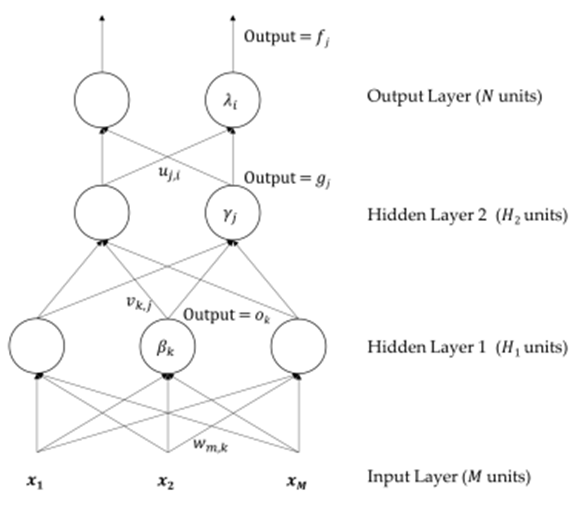
\includegraphics[scale=0.6]{gambar/deeplearning.png}
    % Keterangan gambar yang diinputkan
    \caption{Deep Learning 4 layer}
    % Label referensi dari gambar yang diinputkan
    \label{fig:Deep Learning}
\end{figure}

\subsection{Convolutional Neural Network (CNN)}
Convolutional Neural Network (CNN) merupakan cabang dari Multilayer Perceptron (MLP) yang digunakan untuk
mengolah data dua dimensi. CNN memiliki kedalaman jaringan yang tinggi sehingga CNN termasuk dalam jenis
Deep Neural Network. Perbedaan CNN dengan MLP terdapat pada neuron dimana pada MLP setiap neuron hanya
berukuran satu dimensi, sedangkan CNN setiap neuronnya berukuran dua dimensi. Pada CNN, operasi linier
menggunakan operasi konvolusi[12].

\subsection{Image Processing}
Image Processing atau Pengolahan Citra merupakan teknik dalam pemrosesan gambar dengan input berupa 
citra dua dimensi yang bertujuan untuk menyempurnakan citra atau mendapatkan informasi yang berguna 
untuk diolah menjadi beberapa keputusan. Dalam operasi pemrosesan citra, operasi yang sering dilakukan 
dalam format gambar grayscale. Gambar grayscale didapatkan dari pemrosesan gambar berwarna yang 
didekomposisi menjadi komponen merah (R), hijau (G) dan biru (B) yang diproses secara independen sebagai 
gambar grayscale. Image Processing terbagi menjadi dalam tiga tingkatan[13]:
    \begin{enumerate}
        \item Low-Level Image Processing \\
        Low-Level Image Processing merupakan operasi sederhana dalam pengolahan gambar dimana input dan 
        output berupa gambar. Contoh: contrast enchancement dan noise reduction.
        \item Mid-Level Image Processing \\
        Mid-Level Image Processing merupakan operasi pengolahan gambar yang melibatkan ekstrasi atribut dari 
        gambar input. Contoh: edges, contours dan regions.
        \item High-Level Image Processing \\
        High-Level Image Processing merupakan merupakan kategoriyang melibatkan pemrosesan gambar kompleks 
        yang terkait dengan analisis dan interpretasi konten dalam sebuah keadaan untuk pengambilan keputusan.
    \end{enumerate}

\subsection{Digital Image}
Digital Image merupakan fungsi dua dimensi f(x,y) yang merupakan proyeksi dari bentuk tiga dimensi kedalam 
bentuk dua dimensi dimana x dan y merupakan lokasi elemen gambar atau piksel yang berisikan nilai. Ketika
nilai x,y dan intensitasnya berupa diskrit, maka gambar tersebut dapat dikategorikan sebagai digital
image. Secara matematis, digital image adalah representasi matriks dari gambar dua dimensi menggunakan
piksel. Setiap piksel  diwakili  oleh  nilai  numerik. Untuk  gambar  grayscale,  hanya  memiliki  
satu  nilai dengan kisaran antara 0-255.Pada Gambar 2.5, untuk gambar yang berwarna, memiliki tiga 
nilai yang mewakili merah (R), hijau (G) dan biru (B) yang masing-masing memiliki kisaran nilai yang 
sama antara 0-255. Jika suatu gambar hanya memiliki dua intensitas, gambar tersebut dikenal sebagai 
binary image[13].


  % Konten metodologi
  \section{METODOLOGI}

% Ubah konten-konten berikut sesuai dengan isi dari metodologi

\subsection{Data dan Peralatan/ Data dan Alat Bantu/ Material}

Penelitian ini menggunakan publik dataset yang dikumpulkan dari berbagai sumber untuk setiap kondisi otak, dengan rincian sebagai berikut:

\begin{itemize}
    \item MRI otak normal\\
          Bersumber dari \textbf{IXI Dataset} dengan jumlah citra sebanyak 578.
    \item MRI otak tumor\\
          Bersumber dari \textbf{TCIA Dataset} dengan jumlah citra sebanyak 167.
    \item MRI otak alzheimer\\
          Bersumber dari \textbf{ADNI Dataset} dengan jumlah citra sebanyak x.
    \item MRI otak stroke\\
          Bersumber dari \textbf{ATLAS Dataset} dengan jumlah citra sebanyak x.
\end{itemize}

Penelitian ini menggunakan bahasa pemrograman Python serta device yang bersumber dari cloud service google collaboratory dengan spesifikasi 2vCPU @ 2.2GHz, 13GB RAM, dan 100 GB Memory.

\subsection{Metodologi Penelitian}

    % Contoh input gambar dengan format *.jpg
    \begin{figure} [H] \centering
      % Nama dari file gambar yang diinputkan
      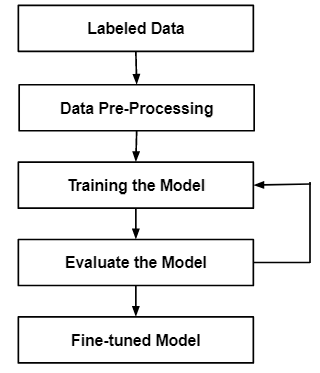
\includegraphics[scale=1]{gambar/Metodologi.png}
      % Keterangan gambar yang diinputkan
      \caption{Metodologi Penelitian}
      % Label referensi dari gambar yang diinputkan
      \label{fig:Metodologi}
    \end{figure}

Pada \emph{Metodologi} yang tertera di Gambar \ref{fig:Metodologi} terdapat 5 tahap dengan detail sebagai berikut:
\begin{outline}
    \1 Labeled Data \\
       Dataset yang digunakan dalam penelitian ini merupakan dataset citra MRI dalam bentuk 3D dengan format NifTI yang sudah memiliki label mengenai kondisi citra otak.
    \1 Data Pre-Processing \\
       Dataset yang sudah diberi label dilakukan pre-processing sebelum masuk ke dalam model agar seluruh data memiliki ukuran dan bentuk yang sama. Pre-process data ini dibagi menjadi 3 bagian yaitu:
       \2 Normalisasi nilai pixel \\
          Nilai pixel dari setiap image dilakukan proses normalisasi agar berada pada range tertentu.
       \2 Normalisasi bentuk image \\
          Bentuk 3D image dilakukan proses normalisasi agar berada pada volume dan bentuk yang sama.
       \2 Data Augmentasi
          Data dirotasi dengan sudut acak untuk menambah jumlah variasi dataset.
    \1 Training Model \\
       Pada penelitian ini model dibuat dengan menggunakan Convolution 3D layer dan Pooling 3D layer. Pada tahap ini akan melakukan percobaan terhadap jumlah layer dan tipe layer model. Selain itu pada tahap ini juga akan dicoba berbagai macam macro function yang berbeda seperti loss function, optimizer function, epoch, dan batch size pada saat training.
    \1 Evaluate Model \\
       Proses evaluasi performa model akan menggunakan confusion matrix yang dengan 4 metric perhitungan, seperti: accuracy, recall, precision, dan F1 Score.
    \1 Fine-Tuned Model \\
       Hasil akhirnya akan berupa sebuah model 3D CNN yang dapat mengklasifikasikan 4 tipe kondisi otak, yaitu: Normal, Alzheimer, Tumor, dan Stroke.
\end{outline}

  % Konten lainnya
  \section{HASIL YANG DIHARAPKAN}

\subsection{Hasil yang Diharapkan dari Penelitian}

Penelitian ini diharapkan dapat menghasilkan sebuah sistem yang dapat mengklasifikasikan 4 tipe kondisi otak, yaitu: Normal, Alzheimer, Tumor dan Stroke dengan menggunakan metode 3D CNN yang dapat digunakan untuk membantu dokter radiologi dalam membuat diagnosa.

\subsection{Hasil Pendahuluan}

Sampai saat ini, kami telah \lipsum[16]

\section{RENCANA KERJA}

% Ubah tabel berikut sesuai dengan isi dari rencana kerja
\newcommand{\w}{}
\newcommand{\G}{\cellcolor{gray}}
\begin{table}[h!]
  \begin{tabular}{|p{3.5cm}|c|c|c|c|c|c|c|c|c|c|c|c|c|c|c|c|}

    \hline
    \multirow{2}{*}{Kegiatan} & \multicolumn{16}{|c|}{Minggu} \\
    \cline{2-17} &
    1 & 2 & 3 & 4 & 5 & 6 & 7 & 8 & 9 & 10 & 11 & 12 & 13 & 14 & 15 & 16 \\
    \hline

    % Gunakan \G untuk mengisi sel dan \w untuk mengosongkan sel
    Data Collection &
    \G & \G & \w & \w & \w & \w & \w & \w & \w & \w & \w & \w & \w & \w & \w & \w \\
    \hline

    Data Pre-Processing &
    \w & \G & \G & \G & \w & \w & \w & \w & \w & \w & \w & \w & \w & \w & \w & \w \\
    \hline

    Pembuatan Model &
    \w & \w & \w & \w & \G & \G & \G & \G & \G & \G & \G & \G & \G & \G & \w & \w \\
    \hline

    Training Model &
    \w & \w & \w & \w & \w & \w & \G & \G & \G & \G & \G & \G & \G & \G & \w & \w \\
    \hline
    
    Evaluasi Model &
    \w & \w & \w & \w & \w & \w & \w & \G & \G & \G & \G & \G & \G & \G & \w & \w \\
    \hline
    
    Pembuatan Laporan &
    \w & \w & \w & \w & \w & \w & \w & \w & \w & \w & \w & \w & \w & \w & \G & \G \\
    \hline

  \end{tabular}
\end{table}

  % Daftar pustaka
  \section{DAFTAR PUSTAKA}
  \renewcommand\refname{}
  \vspace{-2ex}
  \bibliographystyle{unsrtnat}
  \bibliography{pustaka/pustaka.bib}

\end{document}